\documentclass[UTF8]{ctexart}
\usepackage{geometry}
\usepackage{amsmath}
\usepackage{lmodern}
\usepackage{graphicx} %插入图片的宏包
\usepackage{float} %设置图片浮动位置的宏包
\geometry{a4paper,scale=0.8}
\sectionfont{\bfseries\Large\raggedright}

\title{deep-learning笔记}
\author{徐世桐}
\date{}
\begin{document}
\maketitle

% --------------------------------------------------------------------------
% |                                基本定义                                  |
% --------------------------------------------------------------------------
\section{基本定义}

\noindent \textbf{label标签}:输出结果,$\hat{y} $为计算得到的结果,$y$为实际测量结果\\
\textbf{feature特征}:用于预测标签的输入变量,$x^{(i)}_j$为第i组sample第j号特征\\
\textbf{sample样本}:一组特征的取值和对应的标签输出\\
\textbf{batch}:batch size个sample被分为一组,进行向量化的计算,称$B$\\
\textbf{hyperparameter超参数}:人为设定的参数。如样本个数(批量大小batch size)$|B|$,学习率$\eta $。少数情况下通过学习得到\\
\textbf{W 一层layer的权重矩阵} 行数 = 前层节点数,列数 = 当前层节点数
\textbf{全连接层fully-connected layer/稠密层dense layer}:此层所有节点都分别和前一层所有节点连接\\
\textbf{softmax函数}:$softmax(Y) = \frac{exp(y)}{\sum_{y' \in Y} exp(y') } $,将数值输出转化为概率值,1. 值为正 2. 值总和为1\\
\textbf{cross entropy交叉熵}

  定义:分部p 和 分部q 间的 cross entropy $H(p, q) = -E_p(\log (q))$。为 expected value of $log (q)$ with respect to distribution p

  公式:$H(y^{(i)}, \hat{y}^{(i)}) = -\sum_{j\in B}y^{(i)}log(\hat{y}^{(i)})$

  使用:联系两个值概率分部间的差异,即可将数值输出$\hat{y}$和分类结果$y$直接做对比

  \quad 仍可和softmax同时使用,softmax将可能性先转换为正数并和为1,随后使用cross entropy

% --------------------------------------------------------------------------
% |                       linear regression线性回归                         |
% --------------------------------------------------------------------------
\section{linear regression线性回归}
\noindent \textbf{平方代价函数}:$J(\theta ) = \frac{1}{n} \sum_{i = 1}^{n} J^{(i)}(\theta )$,为所有样本误差的平均值\\
\textbf{迭代}:$\theta_i = \theta_i - \frac{\eta}{|B|}\sum_{i\in B} \frac{d J^{(i)}(\theta)}{d \theta_i}$,即对所有sample训练一次,得到label差值,对每一参数减 斜率*学习率 的平均值
  
  当使用平方代价函数:
  
  \quad $\theta_i = \theta_i - \frac{\eta}{|B|}\sum_{i\in B} x^{(j)}_i(x^{(j)}_1\theta_1 + x^{(j)}_2\theta_2 + ... + const - y^{(j)}) = \theta_i - \frac{\eta}{|B|}\sum_{i\in B}x^{(i)}(\hat{y}^{(j)} - y^{(j)})$

  \quad $const = const - \frac{\eta}{|B|}\sum_{i\in B} (x^{(j)}_1\theta_1 + x^{(j)}_2\theta_2 + ... + const - y^{(i)}) = const - \frac{\eta}{|B|}\sum_{i\in B}(\hat{y}^{(j)} - y^{(j)})$

  \quad 对样本i的偏导数向量为$\nabla _{\theta}J^{(i)}(\theta) = 
    \begin{bmatrix}
    x^{(i)}_1 \\
    x^{(i)}_2 \\
    ... \\
    1
    \end{bmatrix}(\hat{y}^{(i)} - y^{(i)})
    $\\
\textbf{交叉熵代价函数}:$J(\theta) = \frac{1}{|B|}\sum_{i\in B} H(y^{(i)}, \hat{y}^{(i)})$\\
\textbf{softmax线性回归}:单层神经网络,使用softmax代价函数\\
\textbf{过拟合问题}

  \textbf{1.权重衰减}:在代价函数中惩罚高权重的值,尽可能使所有权重值减小

  \quad 新代价函数 = $J(\theta) + \frac{\lambda}{2}\sum_{w\in W}w^2$,即 $J(\theta) + \frac{\lambda}{2} * $ 所有权重的平方和。$\lambda$为超参数,决定权重衰减的程度

  \textbf{2.丢弃法}

  \quad 每一权重(不包括const)有p的几率 $\theta' = 0$,有1-p的几率 $\theta' = \frac{\theta}{1-p}$

  \quad 为了得到确切的值,在测试模型时较少使用\\
\textbf{初始化参数}

  \textbf{1.MXNet默认随机初始化}:所有权重$\sim N(0, 1)$的normal distribution,所有const取0

  \textbf{2.Xavier随机初始化}:对一全连接层,输入个数a,输出个数b,则所有参数$\sim U(-\sqrt{\frac{6}{a+b}}, \sqrt{\frac{6}{a+b}})$\\
\textbf{预处理数据集}

  \textbf{1.特征标准化}:$x' = \frac{x - \mu}{\sigma}$,即统计中z值

  \textbf{2.离散值转换成指示特征}:对于一个可取值为A, B, C的离散输入值,转换成3个数值输入。即如果原输入为A,转换后3个数值输入为1,0,0。原离散值为B则转换后为0,1,0\\
\textbf{结构}
  
  - 将训练集分组,每组batch\_size个sample。
  
  - 对这个batch的数据进行向量化计算,计算loss,斜率,调用优化函数。

  - 即每一batch使用相同的权重 偏差。一次训练一共只遍历一次所有sample,共$\frac{sample\_size}{|B|}$次向量化计算\\
\textbf{activation function只出现在hidden layer的输出,输出层无需activation function}


% --------------------------------------------------------------------------
% |                convolutional neural network卷积神经网络                  |
% --------------------------------------------------------------------------

\section{convolutional neural network卷积神经网络}
\noindent \textbf{互相关运算}:

  输入一个二维数组,和\textbf{二维核kernel}进行互相关运算,得到二维数组

  \textbf{二维核/卷积核/filter 过滤器}:在输入数组上滑动,每次和二维数组矩阵一部分按元素相乘 求和,作为输出矩阵的元素\\
\textbf{二维卷积层}:

  将输入和卷积核做互相关运算,结果加上const作为输出\\
\textbf{特征图}:输出矩阵可看做是输入矩阵的表征,称特征图\\
\textbf{感受野receptive field}:
  
  对输出矩阵一元素x,所有可能影响其值的输入矩阵元素称感受野

  感受野可能大于实际输入的矩阵边界\\
\textbf{填充padding}:
  
  在输入矩阵外侧添加全零元素,使得输出矩阵的维度增加,由于可用的感受野增加。

  常使用奇数kernel,添加$\lfloor \frac{kernel}{2}\rfloor $的填充,使得输出矩阵和输入矩阵纬度一样\\
\textbf{步幅stride}:

  定义每次感受野向左/向下移动的纬度\\
\textbf{多通道输入输出}:

  当输入的数据包含多个矩阵,即多通道输入,例:RGB图像有3个输入通道

  对$c_i$输入, $c_o$输出的卷积层,kernel shape为($c_o$, $c_i$, 行数,列数)

  \quad 每一输入通道有唯一的kernel ($c_i$, 行数,列数)对应,进行互相关运算后结果矩阵相加,作为一条输出通道的结果

  \quad 多组($c_i$, 行数,列数)分别产生输出通道的结果矩阵,则有$c_o$条输出通道\\
\textbf{池化层}:
  
  作用:1 为了防止当输入变化时,输出立即随之更改。2 减少计算量

  池化窗口,同卷积层的感受野。限定某块输入被同时考虑,同样有stride,可对输入padding

  \quad 1. 最大池化层:取池化窗口内最大的输入

  \quad 2. 平均池化层:取池化窗口平均值

  \textbf{多输入通道间池化结果不相加,即 输入通道数 = 输出通道数}\\
\textbf{LeNet卷积神经网络}

  \textbf{1.使用2组 卷积计算层 激活函数层 池化层}

  \quad 输出通道数分别为6,16。卷积层 kernel 为(5, 5), 步幅为1, 无padding

  \quad 激活函数层 对每一元素做sigmoid

  \quad 池化层 窗口(2, 2),步幅为2

  \textbf{2.使用3组全连接层}

  \quad 节点数120 84 10,使用sigmoid激活函数

  \quad 将(批量大小, 通道数, height, width) 看做 (批量大小,通道数 * height * width)处理\\
\textbf{AlexNet深度卷积神经网络}:

  除输出层和丢弃层,全部使用relu做激活函数

  \textbf{卷积部分}
  
  \quad - 2组包含pooling的卷积计算
  
  \quad \texttt{nn.Conv2D(96, kernel\_size=11, strides=4, activation='relu')}

  \quad \texttt{nn.MaxPool2D(pool\_size=3, strides=2)}

  \quad \texttt{nn.Conv2D(256, kernel\_size=5, padding=2, activation='relu')}

  \quad \texttt{nn.MaxPool2D(pool\_size=3, strides=2)}
  
  \quad - 3组仅pooling一次的卷积计算,高输出通道,低卷积窗口
  
  \quad \texttt{nn.Conv2D(384, kernel\_size=3, padding=1, activation='relu')}
  
  \quad \texttt{nn.Conv2D(384, kernel\_size=3, padding=1, activation='relu')} 
  
  \quad \texttt{nn.Conv2D(256, kernel\_size=3, padding=1, activation='relu')}
  
  \quad \texttt{nn.MaxPool2D(pool\_size=3, strides=2)}

  \textbf{全连接层部分}
  
  \quad - 两hidden layer全连接层使用丢弃法

  \quad \texttt{nn.Dense(4096, activation="relu"), nn.Dropout(0.5)}
  
  \quad \texttt{nn.Dense(4096, activation="relu"), nn.Dropout(0.5)}
  
  \quad \texttt{nn.Dense(10)} // 根据需求改变输出层节点,原论文为1000\\
\textbf{VGG使用重复元素网络}

  \textbf{VGG基础块}

  \quad 数个(3, 3)kernel 1填充卷积层 + 1个(2, 2)窗口 2步幅池化层

  VGG 神经网络由 数个VGG块 + 数个全连接层 组成

  例:\textbf{VGG-11}
  
  \quad 包含结构为(1, 64) (1, 128) (2, 256) (2, 512) (2, 512) 5层VGG块

  \quad \quad (n, m) 代表此VGG块使用n层卷积层,各有m通道
  
  \quad 和3层全连接层,实现同AlexNet的全连接层部分
  
  \quad 共8层卷积层+3层全连接层,所以称VGG-11\\
\textbf{NiN神经网络}

  \textbf{NiN块}

  \quad 1个自定义卷积层 + 2层 (1, 1)kernel 卷积层,3层卷积层都不包含池化层,都有同样通道数

  \quad 自定义卷积层可设置kernel,步幅,填充。(1, 1)除了通道数可设置,其余固定为默认值

  NiN神经网络有多组 (NiN块 + 池化层) 每一NiN块后有池化层
  
  例:\textbf{NiN模型}

  \quad - NiN块部分

  \quad \texttt{nin\_block(96, kernel\_size=11, strides=4, padding=0)}

  \quad \texttt{nn.MaxPool2D(pool\_size=3, strides=2)}

  \quad \texttt{nin\_block(256, kernel\_size=5, strides=1, padding=2)}

  \quad \texttt{nn.MaxPool2D(pool\_size=3, strides=2)}

  \quad \texttt{nin\_block(384, kernel\_size=3, strides=1, padding=1)}

  \quad \texttt{nn.MaxPool2D(pool\_size=3, strides=2)}

  \quad - 在NiN块部分结束后加入丢弃层

  \quad \texttt{nn.Dropout(0.5)}

  \quad - 转化为对应分类个数的输出

  \quad \texttt{nin\_block(10, kernel\_size=3, strides=1, padding=1)}

  \quad \texttt{nn.GlobalAvgPool2D()} // 全局平均池化层,每一通道取矩阵所有元素的平均值

  \quad \texttt{nn.Flatten()} // 将四维的输出转成二维的输出,其形状为(批量大小, 10)\\
\textbf{GoogLeNet含并行结构神经网络}

  \textbf{Inception块}
  \begin{figure}[H] %H为当前位置,!htb为忽略美学标准,htbp为浮动图形
    \centering %图片居中
    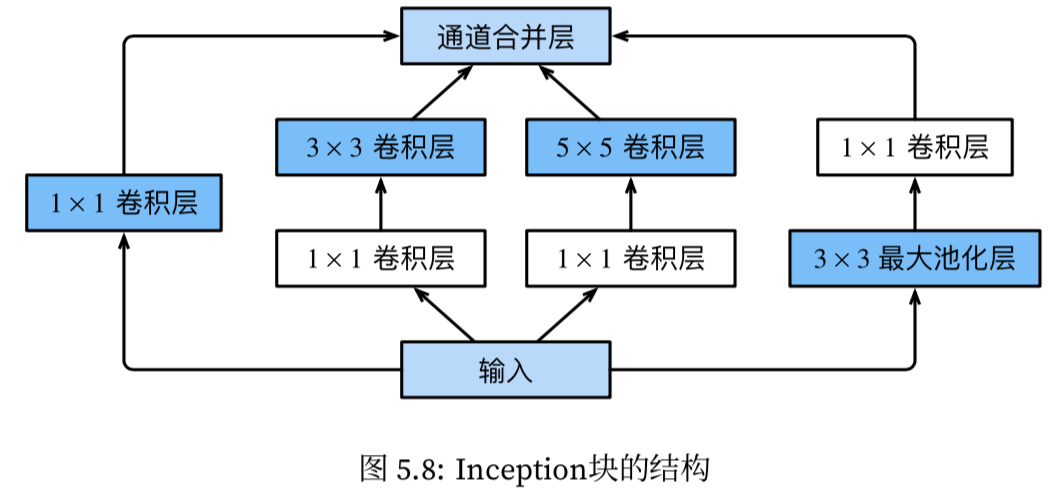
\includegraphics[width=0.6\textwidth]{note_images/inception_block.png} %插入图片,[]中设置图片大小,{}中是图片文件名
  \end{figure}

  \quad 结构表示:($n_1$, ($n_{21}$, $n_{22}$), ($n_{31}$, $n_{32}$), $n_4$) 
  
  \quad \quad 第一线路使用$n_1$通道
 
  \quad \quad 第二线路第一卷积层使用$n_{21}$通道,第二层卷积层使用$n_{22}$通道 1填充
 
  \quad \quad 第三线路第一卷积层使用$n_{31}$通道,第二层卷积层使用$n_{32}$通道 2填充
  
  \quad \quad 第四线路第一池化层使用(3, 3)窗口 1填充,第二层卷积层使用$n_4$通道

  \quad 每一卷积层都使用relu激活函数

  \quad 所有层输出作为不同通道结果,即最终有$n_1 + n_{22} + n_{32} + n_4$通道

  GoogLeNet结构:

  \quad 5个串联模块,每一卷积层使用relu激活函数,每一模块间使用 步幅2 (3, 3)窗口 1填充 池化层

  \quad 1. 64通道(7, 7)kernel 2步幅 3填充卷积层 + 池化层

  \quad 2. 64通道(1, 1)kernel卷积层 + 64 * 3通道(3, 3)kernel 1填充卷积层 + 池化层

  \quad 3. 串联2 inception 块 + 池化层,分别有结构

  \quad \quad (64, (96, 128), (16, 32), 32)

  \quad \quad (128, (128, 192), (32, 96), 64)

  \quad 4. 串联5 inception 块 + 池化层

  \quad \quad (192, (96, 208), (16, 48), 64)

  \quad \quad (160, (112, 224), (24, 64), 64)

  \quad \quad (128, (128, 256), (24, 64), 64)

  \quad \quad (112, (144, 288), (32, 64), 64)

  \quad \quad (256, (160, 320), (32, 128), 128)

  \quad 5. 串联2 inception 块 + 全局平均池化层

  \quad \quad (256, (160, 320), (32, 128), 128)

  \quad \quad (384, (192, 384), (48, 128), 128)

  \quad 6. 全连接层,节点数和分类类别数相

% --------------------------------------------------------------------------
% |                              优化方法                                   |
% --------------------------------------------------------------------------
\section{优化方法}
\noindent \textbf{批量归一化 batch normalization}

  \textbf{1. 对全连接层做批量归一}

  \quad 处于 输入的仿射变换 和 激活函数间,即 输出 = $\phi (BN(x))$ 

  \quad 1. 对于批量仿射 $x = Wu + b$,求标准化$\hat{x}_i = \frac{{x_i} - \mu}{\sqrt{\sigma^2 + \varepsilon }}$。$\mu $和 $\sigma$都为此组仿射变换的结果

  \quad 2. $BN(x) = \gamma * \hat{x}_i + \beta $,$\gamma$拉伸 $\beta$偏移。* + 为按元素加法 乘法

  \textbf{2. 对卷积层做批量归一}

  \quad 处于 卷积计算 和 激活函数 间,卷积计算 -> 批量归一 -> 激活函数 -> 池化层

  \quad 各通道独立计算,各有独立拉伸$\gamma$ 偏移$\beta$。
  
  \quad $\sigma$, $\mu$为此通道 一批量内 所有矩阵 的所有元素 的总体方差,平均值

  \quad 得到$\sigma$, $\mu$后对此通道此批量内所有元素求标准化

  \quad 最终对此通道 每一sample标准化的结果拉伸 偏移\\
\textbf{ResNet残差网络}

  \textbf{残差块}

  \quad 训练时期望输出为f(x) - x,而非直接使用f(x)期望输出。得到f(x) - x后+x得到f(x)

  \quad 1. 卷积层(批量归一) + relu + 卷积层(批量归一) 得到$f(x) - x$
  
  \quad 2. $f(x) - x$+(1, 1)卷积层对(x)卷积结果 + relu激活函数
  
  \quad \quad 第一卷积层:(3, 3)kernel 1填充 (通道数 步幅自定义)

  \quad \quad \quad 第234组残差组 第一残差块 第一卷积层步幅为2,否则为1

  \quad \quad 第二卷积层:(3, 3)kernel 1填充 1步幅 (通道数自定义)

  \quad \quad (1, 1)卷积层:(通道数 步幅自定义) 

  \quad \quad \quad 第234组残差组 第一残差块使用(1, 1)卷积层,步幅为2,否则直接+x

  \quad \quad 3层卷积层通道数共享同一自定义值,\textbf{要求2层卷积层输入输出通道数一致}

  ResNet-18模型:共18卷积层

  \quad 1. 64通道(7, 7)kernel 2步幅 3填充 批量归一卷积层 + (3, 3)窗口 2步幅 1填充最大池化层

  \quad 2. 4组 残差块,每组包含多个残差块

  \quad \quad 第一组 2个残差块 输出通道数和1中输出通道数一致
  
  \quad \quad 第二三四组 各2个残差块 输出通道数为前一层通道数$*2$

  \quad 3. 全局平均池化层 + 对应输出结果数全连接层\\
\textbf{DenseNet稠密连接网络}

  类似ResNet残差网络,+x步变为concat x连在输出结果后,即x直接传向下一层

  \textbf{稠密块}

  \quad 多组(批量归一 + relu + (3, 3)kernel 1填充卷积层 + concat x) 卷积层通道数相同

  \quad concat操作为在通道纬度的concat,即输入x作为额外输出通道。

  \quad 增长率 = 输出通道 - 输入通道 = 卷积层通道数

  \textbf{过渡层}

  \quad 批量归一 + relu + (1, 1)卷积层 + (2, 2)窗口 2步幅平均池化层
  
  \quad 使用(1, 1)卷积层减小通道数,2步幅平均池化层减小矩阵大小

  \quad \quad 卷积层通道数 = 输出通道数 / 2

  DenseNet模型

  \quad 1. 64通道(7, 7)kernel 2步幅 3填充 批量归一卷积层 + (3, 3)窗口 2步幅 1填充最大池化层

  \quad 2. 4组稠密块,由3个过渡层分隔

  \quad \quad 4层稠密块卷积层数可以不相同

  \quad 3. 批量归一 + relu + 全局平均池化层 + 对应输出结果数全连接层

% --------------------------------------------------------------------------
% |                             循环神经网络                                 |
% --------------------------------------------------------------------------
\section{循环神经网络}

\noindent 记录数据状态,根据以往状态和当前输入决定输出\\
\textbf{n阶马尔科夫链}:一个词的出现仅和前n个词有关\\
\textbf{语言模型}:词序($w_1$, $w_2$, ..., $w_T$)的出现可能性为

  $P(w_1, w_2,...,w_T)\approx \prod_{t=1}^{T} P(w_t|w_{t-(n-1)},...,w_{t-1})$

  称n元语法,每一$w_t$为一时间步中出现的词\\
\textbf{循环神经网络}

  隐藏层$H_t = \phi(X_tW_{xh} + H_{t-1}W_{hh} + b_h)$

  \quad $H_{t-1}W_{hh}$项将隐藏层前一次输出纳入此次计算

  输出$O = HW_{hq} + b_q$\\
\textbf{处理语言模型}:将每一文字转化为索引,使用索引做训练参数集\\
\textbf{采样方式}:

  $BATCH_SIZE$ 每次采集的样本数
  
  $NUM_STEPS$ 每个样本包含的时间步数,

  \textbf{1 随机采样}:

  \quad [1 2 3 4] [5 6 7 8] [9 10 11 12] [13 14 15 16]

  \quad 将所有样本分为头尾相连的组,每组有相等可能性被取值,每次随机取BATCH\_NUM组

  \quad 训练来自不同批量的样本时不能将前一次隐藏层结果纳入计算
  
  \textbf{2 相邻取样}:

  \quad [1 2 3 4    ] [5 6 7 8    ] [9 10 11 12 ] [13 14 15 16]

  \quad [17 18 19 20] [21 22 23 24] [25 26 27 28] [29 30 31 32]

  \quad 将样本填入BATCH\_NUM行矩阵,再分为(BATCH\_NUM, NUM\_STEPS)的小矩阵,每次每个小矩阵有等可能性被选择
  
  \quad 仅需在训练一开始初始化隐藏层结果,而非在每一批量开始初始化
  

  
% --------------------------------------------------------------------------
% |                       Deep Learning 第6章笔记                           |
% --------------------------------------------------------------------------

\section{Deep Feedforward Network (Deep Learning 第6章笔记)}
\noindent \textbf{SVM支持向量机}

  仍通过$w^Tx+b$得到输出,输出仅表示identity,正值说明有identity,负值说明没有

  依据:一个平面的公式为$\beta_0+\beta_1x_1+\beta_2x_2=0$,则当计算$w^Tx+b$得到值后,>0则为平面上方的数据点,<0为下方数据点\\
\textbf{kernel trick}

  kernel method将数据集表示成相近的两个数据点一组的集合$(x_i, x_j)$,kernel method将一对数据变为单一数据点$x=k(x_i, x_j)=\langle \phi (x_i), \phi (x_j)\rangle $

  kernel method使用$\phi $转换数据的纬度,而点乘 化简后无需先计算$\phi (x_i), \phi (x_j)$即可得到新数据点$x$\\
\textbf{manifold hypothesis:}

  当训练数据集合包含大量无规律的数据,则将其中大部分视为无效数据,并只关心落在一个manifold上的数据。

  例:生成图像 文字 声音时数据大多很集中,当像素文字随机分布时生成图像大多无意义\\
\textbf{deep feedforward network/feedforward neural network/multilayer perceptrons MLP:}

  找到$\theta$使得$f(x; \theta )$ 最接近数据y值。$f^*$为最理想的f,即$f^*(x) = y$。$\theta $可为多个参数,如$f(x; w, b) = x^Tw+b$

  $f^*(x) = f^{(3)}(f^{(2)}(f^{(1)}(x)))$,$f^{(1)}$为network第一层。每一$f^{(i)}(x) = \phi (x; \theta )^Tw$

  \textbf{神经网络}

  \quad 1. 结构:

  \quad \quad 输入层没有weight,第一hidden layer得到所有输入层的值。

  \quad \quad hidden layer和输出层所有输出都为0/1,非连续的值

  \quad 2. 一层hidden layer计算方法:$ f^{(i)}(x; W, c) = \sigma (W^Tx + c)$

  \quad \quad x 为前一层的输出向量,输入层x即为训练参数向量。 

  \quad \quad c 为此层常数向量

  \quad \quad z = $W^Tx$为一层hidden layer对输入取得的中间值向量,称logit。a = $\sigma (z + c)$为对z + c每一元素取$\sigma $的结果向量,a即此层的输出。

  \quad \quad W 为此层参数矩阵,行数 = 前层节点数,列数 = 当前层节点数

  \quad \quad X 为多个参数点的训练集中前一层的输出矩阵,行数为数据点个数,列数为前一层节点数

  \quad \quad $XW$ 当W对参数集矩阵操作时,每行向量$z_{i}^T$此时为一层hidden layer各节点对第i参数点的中间值向量。对每行+$c^T$并分别取$\sigma $得到输出矩阵,$a_{ij}$为当使用第i个参数点时此层第j节点的输出

  \textbf{cross entropy}

  \quad 分部p 和 分部q 间的 cross entropy $H(p, q) = -E_p(\log (q))$。为 expected value of $log (q)$ with respect to distribution p

  \textbf{cost function}

  \quad 当使用maximum likelihood估计参数时,cost function$J(\theta )$为 训练输入参数的分部 和 训练结果参数的分部 间cross-entropy: $J(\theta ) = -E_{x, y\sim training\_dataset}(log (p_{model}(y | x)))$

  \quad \quad 对于每一在训练集内的(x, y),求$log (p_{model}(y | x))$, 并求expected value。$p_{model}(y | x)$ 即训练得到的y关于x的分部

  \quad \quad 例:当model为$y = N(f(x; \theta), 1)$正则分部时,$J(\theta) = -E_{x, y\sim data}(y - f(x;\theta))^2 + const$

  \textbf{output layer}

  \quad 当输出层的结果和不为1时,代表数据没有被准确分到某一类中,使用exponentiation and normalisation

  \quad \quad normalisation后结果 $p = \frac{\tilde{p} }{\sum \tilde{p'} } $,为$\tilde{p} $在所有结果中占的比例。$\tilde{p} $为未normalise 值

  \quad 假设输出层结果$\tilde{P} (y | x)$ 有 $log(\tilde{P} (y | x)) = yz$

  \quad \quad $\tilde{P} (y | x) = exp(yz)$

  \quad \quad $P (y | x) = \frac{exp(yz)}{\sum_{y' = 0}^{1} y'z } $,称\textbf{softmax function}

  \quad \quad $P (y | x) = \sigma ((2y - 1)z)$,y,y'为训练目标结果,所以$\sum_{y' = 0}^{1} $包含所有y'

  \quad 对softmax function使用log likelihood原因:log $softmax(z)_i = z_i - log\sum_j exp(z_j)$。

  \quad \quad 当$z_i$为dominant,并对应期望的输出项。log $softmax(z)_i$ = 0。则此项不产生高cost,否则产生cost。

  \textbf{hidden unit}

  \quad \quad 代表一个hidden layer节点的激发函数。

  \quad \quad 1. rectified linear unit: $g(x) = max(0, x)$

  \quad \quad \quad 无法用于gradient based learning,由于一阶导为0

  \quad \quad \quad 基于rectified linear unit的优化:$g(x) = max(0, x) + a*min(0, x)$

  \quad \quad \quad \quad a = -1:absolute value rectifier

  \quad \quad \quad \quad a 为极小值:leaky ReLU

  \quad \quad \quad \quad a 为可学习值:Parametric ReLU, PReLU

  \quad \quad 2. Maxout units

  \quad \quad \quad 将x分为多组,每组h(x) 为组内最高值

  \textbf{backward propagation}

  \quad 一种计算gradient的方法,区别于使用gradient进行学习的stochastic gradient descent

  \quad 算法:
  \begin{figure}[H] %H为当前位置,!htb为忽略美学标准,htbp为浮动图形
    \centering %图片居中
    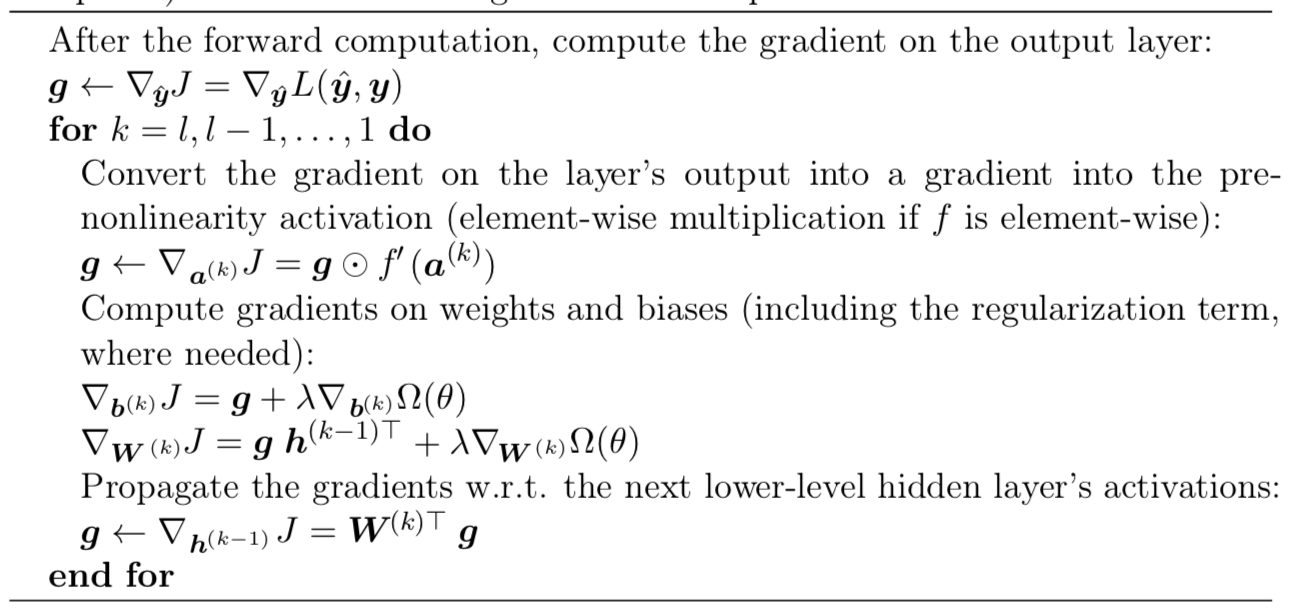
\includegraphics[width=0.6\textwidth]{note_images/backprop_algo.png} %插入图片,[]中设置图片大小,{}中是图片文件名
  \end{figure}

  
\end{document}
